\documentclass[10pt]{article}
\usepackage[utf8]{inputenc}
\usepackage[T1]{fontenc}
\usepackage{geometry}
\geometry{letterpaper, margin=0.55in}
\usepackage{graphicx}
\usepackage{booktabs}
\usepackage{caption}
\usepackage{enumitem}
\usepackage{hyperref}
\usepackage{xcolor}

\setlength{\parskip}{3pt}
\setlength{\parindent}{0pt}

\title{\vspace{-1.2cm}\textbf{ProverbGap MCQ --- State of Work \& OpenRouter Quota Request}}
\author{Sunday Aspita Abraham \quad | \quad 2026 Fatima Fellow \quad | \quad 22 June 2026}
\date{}

\begin{document}

\maketitle
\vspace{-0.6cm}

\section*{1. What we are building}
ProverbGap MCQ is a cross-lingual benchmark that tests whether language models truly understand proverbs in English, Arabic, and Yoruba, or whether they are just exploiting surface shortcuts. We generate multiple-choice questions where the model must pick the correct English meaning of a proverb from three tempting distractors. The twist is that the distractors are generated adversarially and then audited by a blind committee of other models that see only the four answer choices --- not the proverb itself.

\section*{2. Why it matters}
Proverbs are a good stress-test for LLMs because their meaning is rarely literal and often culture-specific. A model can score well on standard reading comprehension and still fail a proverb. Existing benchmarks usually release MCQs without validating whether the wrong options are genuinely tempting. We are trying to fix that, especially for low-resource languages like Yoruba where good evaluation data is scarce. This work builds on my track record of building low-resource NLP benchmarks, including an accepted oral presentation at Data Science Africa 2026 and a published PMLR paper on domain adaptation for African agriculture.

\section*{3. What we used the OpenRouter API for}
\begin{itemize}[leftmargin=0.5cm, itemsep=1pt]
    \item \textbf{Distractor generation:} multiple generator models (Qwen, Gemma, Gemini) produce candidate wrong options.
    \item \textbf{Blind audit:} a disjoint committee of models (Llama, Mistral, Gemma, DeepSeek) votes on which option is correct without seeing the proverb.
    \item \textbf{Gold-meaning curation:} a small model rewrites literal/awkward glosses into natural English.
    \item \textbf{LLM fallback test:} an experimental distractor generator that produces proverb-specific hard negatives on demand.
\end{itemize}

\section*{4. Progress so far}
Our cleanest scaled run so far is v68 (N=5): 15 proverbs, 4 prompt variants, 3 generators, 180 MCQs, costing \$0.85. Keys were perfectly balanced across A/B/C/D and there were zero exact duplicates. The blind committee was only 56.7\% accurate overall --- only modestly above the 25\% random baseline --- which means the distractors are genuinely tempting. Arabic and Yoruba consensus accuracy stayed near 50--53\%, exactly the difficulty range we want for a hard benchmark.

\begin{table}[h]
\centering
\small
\caption*{Table 1. OpenRouter cost progression across recent runs.}
\begin{tabular}{@{}ccccc@{}}
\toprule
Version & Date & Proverbs & MCQs & Cost (USD) \\
\midrule
v58 & 2026-06-20 & 3 & 45 & \$0.22 \\
v61 & 2026-06-20 & 3 & 36 & \$0.19 \\
v65 & 2026-06-21 & 3 & 36 & \$0.19 \\
v68 & 2026-06-22 & 15 & 180 & \$0.85 \\
v70 (partial) & 2026-06-22 & 15 & 83* & \$0.42* \\
\bottomrule
\end{tabular}
\\[2pt]
\footnotesize *v70 stopped when the API key hit its monthly budget.
\end{table}

\begin{figure}[h]
\centering
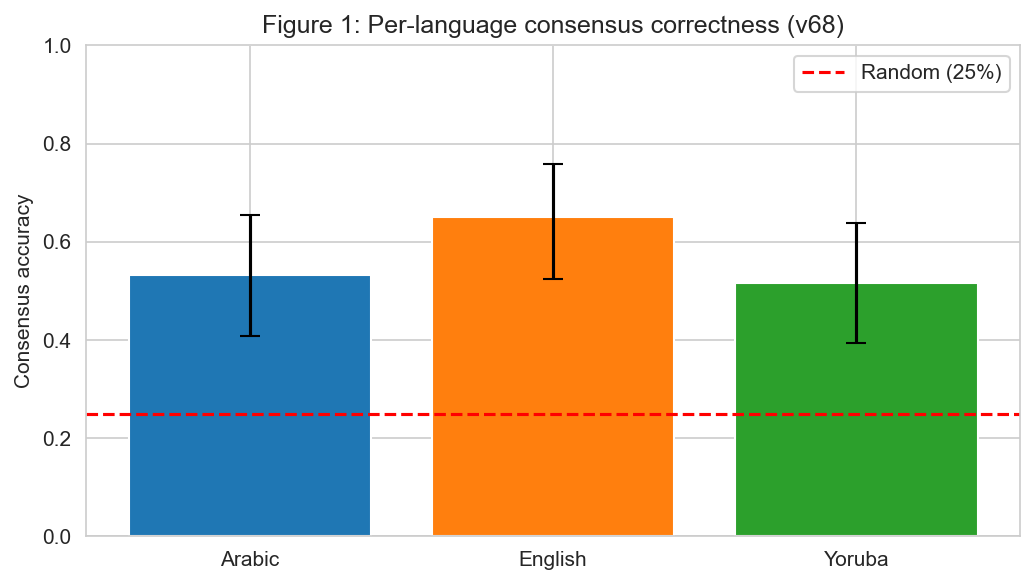
\includegraphics[width=0.45\textwidth]{figures/fig1_per_language_consensus_accuracy.png}
\caption*{Figure 1. Consensus accuracy by language (v68, N=5). English is easiest; Arabic and Yoruba are near random, showing the distractors are hard.}
\end{figure}

\begin{figure}[h]
\centering
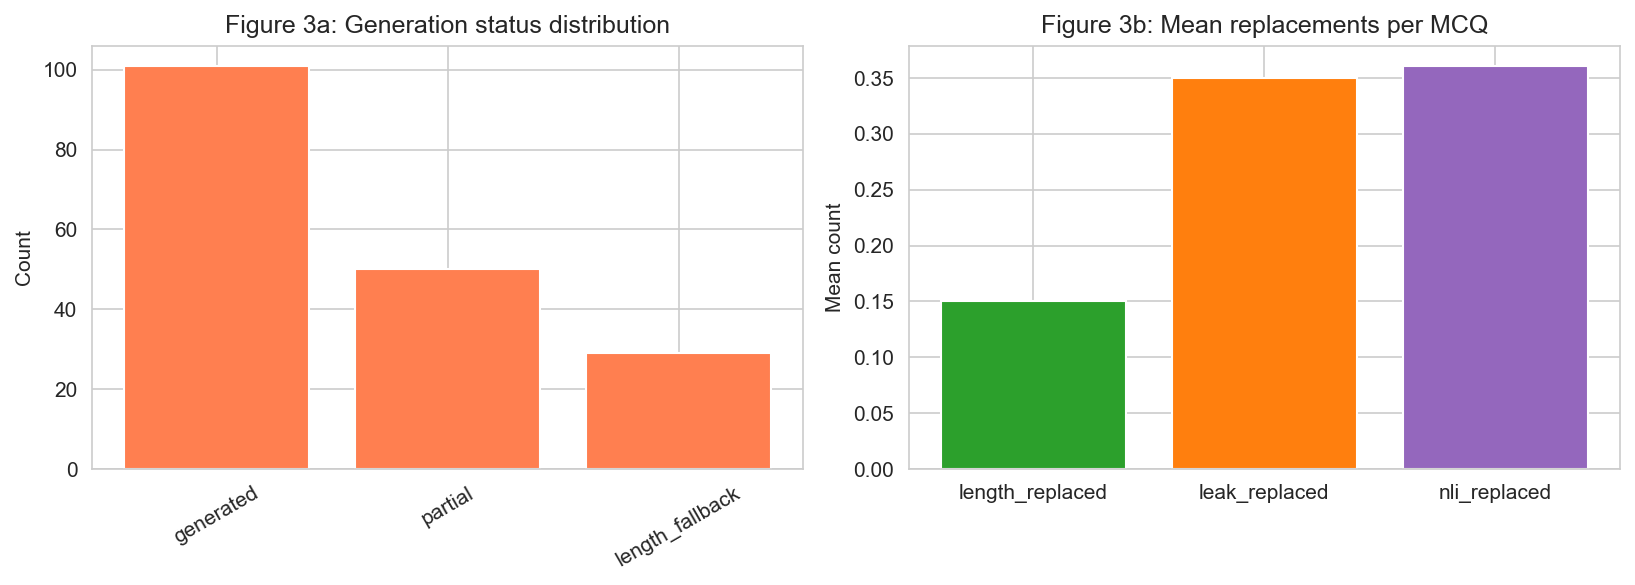
\includegraphics[width=0.45\textwidth]{figures/fig2_generation_status_and_repairs.png}
\caption*{Figure 2. Generation status and mean repairs per MCQ. 44\% of items needed fallback repairs; NLI/leak filters are the main drivers.}
\end{figure}

\section*{5. The bottleneck we hit}
The main problem is our corpus-based fallback sampler. When the NLI paraphrase or correct-meaning-leak filter rejects a model-generated distractor, the pipeline pulls a replacement from other proverbs' meanings. Those replacements are often plausible enough for auditors to agree on, but wrong. In v68, 44\% of items needed fallback repairs and 28\% became high-consensus-wrong (3 of 4 auditors agreed on the wrong answer).

We attempted v70 with the LLM-based fallback generator at the same N=5 scale (15 proverbs total), but the run stopped after 83 MCQs because the OpenRouter API key hit its monthly budget. Once the cap was reached, every further model call returned HTTP 403 ``Budget limit exceeded'', the generator pool exhausted its substitutes, and the run crashed with ``No active generators remaining''. Without more quota we cannot scale to N=15 per language or confirm whether the LLM fallback fixes the HCW problem.

\begin{figure}[h]
\centering
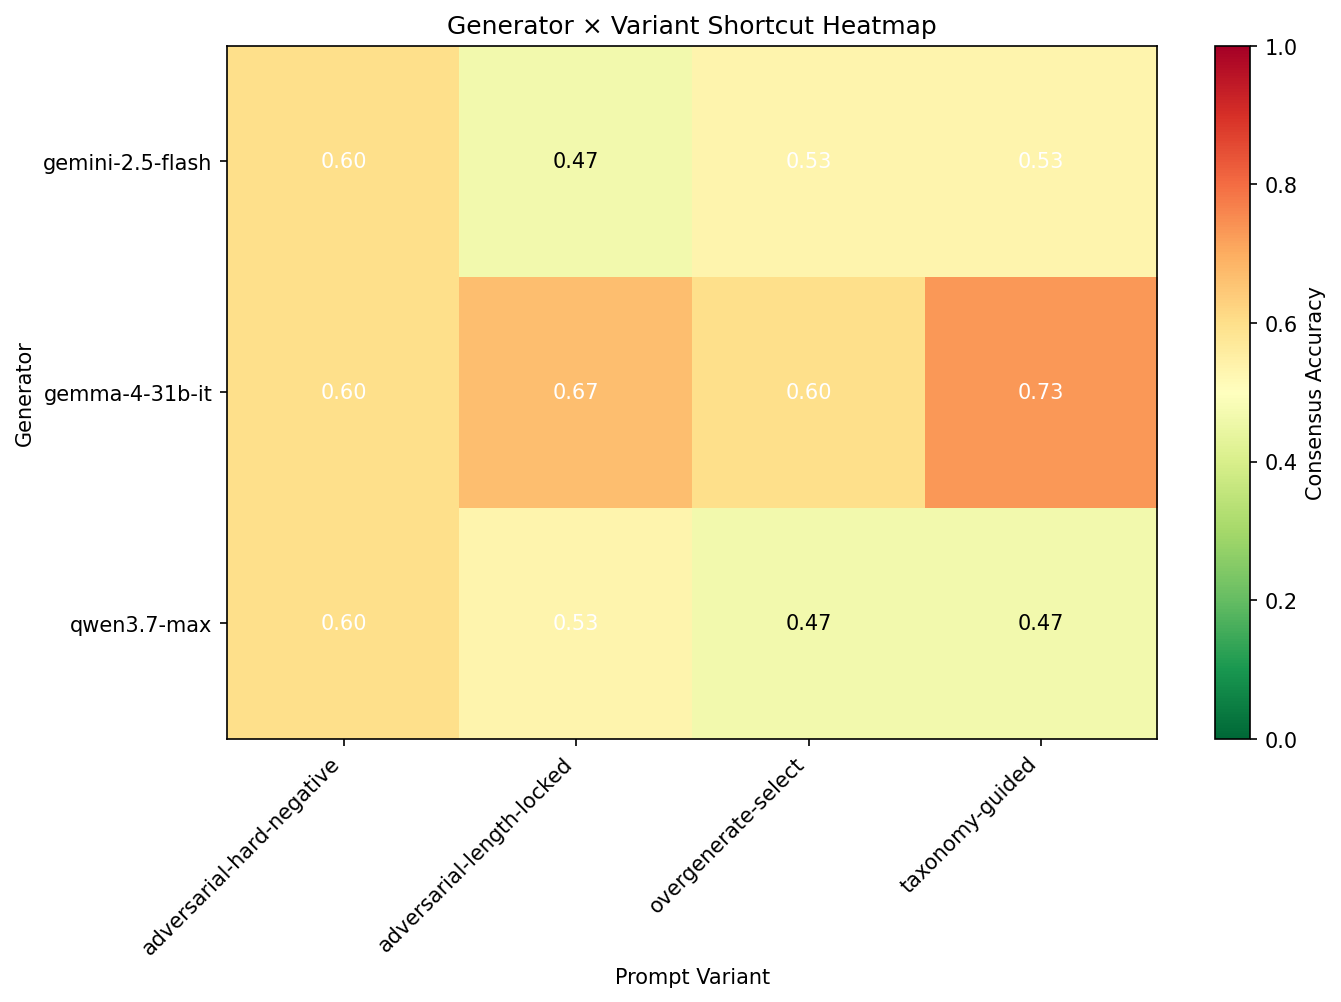
\includegraphics[width=0.45\textwidth]{figures/fig3_generator_variant_accuracy_heatmap.png}
\caption*{Figure 3. Generator $\times$ variant accuracy heatmap (v68). Performance varies by model and prompting strategy.}
\end{figure}

\begin{figure}[h]
\centering
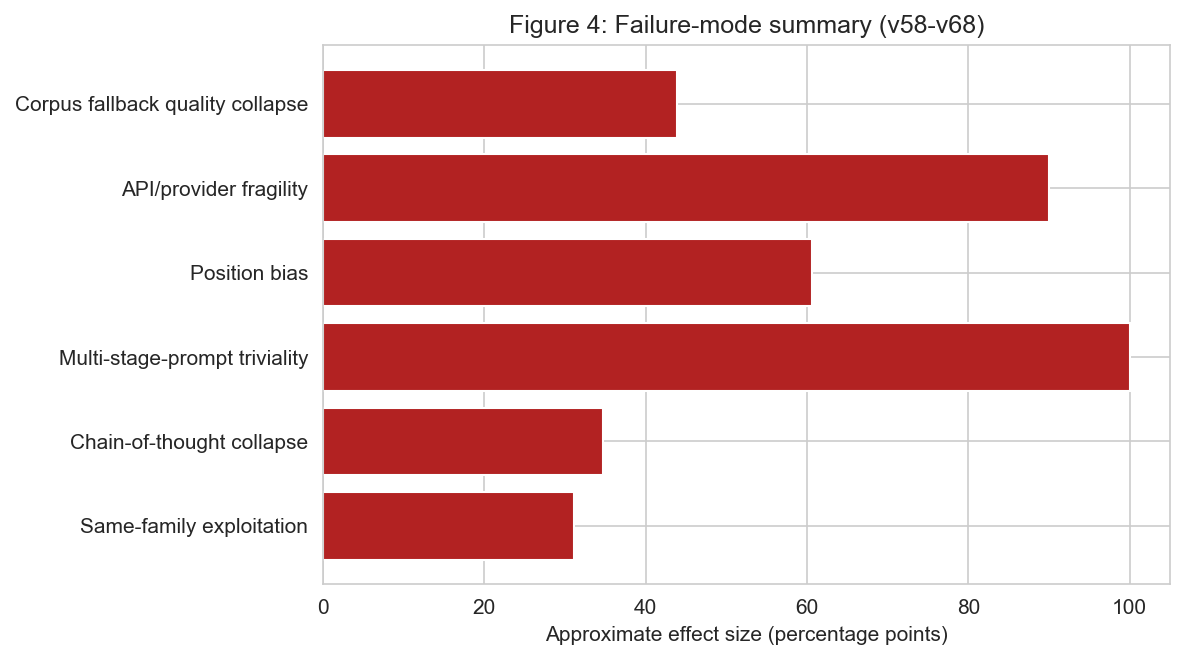
\includegraphics[width=0.45\textwidth]{figures/fig4_failure_mode_summary.png}
\caption*{Figure 4. Failure modes documented across v58--v68. Each is a reproducible pipeline weakness we treat as a contribution.}
\end{figure}

\section*{6. What we need}
We are requesting an increase in the OpenRouter monthly quota. Based on v68 costs, we estimate about \$10--15 in additional API credit would let us complete v70 at N=15 per language (45 proverbs total, roughly 3$\times$ the v68 cost of \$0.85, so about \$2.60), run the LLM-fallback ablation at the same N=5 scale (\$2--3), and generate the 60-item human-validation sample. This will give us a rigorous, audited dataset and a clear answer on whether the fallback bottleneck can be solved.

\section*{7. Next steps if quota is increased}
\begin{itemize}[leftmargin=0.5cm, itemsep=1pt]
    \item Finish v70 N=15 generation and audit ($\sim$2--3 Kaggle runs).
    \item Run human validation: 60 MCQs, 20 per language, 2--3 native speakers per language.
    \item Draft and submit a methodology paper to EACL 2027 ARR (deadline 3 August 2026).
    \item Release the pipeline, audit logs, and dataset as a reproducible testbed.
\end{itemize}

\end{document}
